\documentclass[11pt]{article}

% Final (camera-ready) version: omit the "review" option to drop line numbers.
\usepackage[final]{acl}

\usepackage{times}
\usepackage{latexsym}
\usepackage[T1]{fontenc}
\usepackage[utf8]{inputenc}
\usepackage{microtype}
\usepackage{inconsolata}
\usepackage{graphicx}
\usepackage{booktabs}
\usepackage{amsmath}
\usepackage{amssymb}
\usepackage{xcolor}
\usepackage{hyperref}

\newcommand{\projectrepolink}{\url{https://github.com/avih7531/headline-structure-analysis}}

\title{Structural Patterns in News Headlines:\\A Computational Linguistic Analysis Using NLP}

\author{Victor Derani \and Avi Herman \and Kylie Lin \\
  Department of Computer Science \\
  New York University \\
}

\begin{document}
\maketitle

\begin{abstract}
We analyze the syntactic and structural patterns of news headlines using NLP. Our pipeline collects headlines from RSS feeds, parses them with spaCy, and feeds the parses into a transparent rule-based classifier. The classifier assigns each headline a primary structural label (question, passive, coordination, noun-phrase fragment, simple clause, or other) plus a four-dimensional style profile (lead frame, agency style, density band, rhetorical mode). Our claim is simple: headlines are not free-form prose but reproducible syntactic products whose form is recoverable, structurally constrained, and stylistically decomposable.

On a manually annotated gold-standard set of 464 headlines, the classifier reaches \textbf{0.806 accuracy} and \textbf{0.675 macro F1} on the held-out test split. That beats a majority baseline by $+16.3$ accuracy points (macro F1 $0.130 \rightarrow 0.675$) and a random baseline by $+34.7$ points. A 5-seed split-stability sweep places the structure test macro F1 mean at $\mathbf{0.568 \pm 0.076}$, making the size of ``split luck'' explicit. Style dimensions decompose cleanly: framing and density are nearly perfectly recoverable (test macro F1 $1.000 / 1.000$), while agency and rhetorical mode are harder ($0.428 / 0.820$).

The takeaway: headline writing follows recoverable rules, and interpretable, parse-grounded methods capture them well --- no opaque neural models required. The framework supports summarization, style auditing, and media-framing analysis, and is exposed through an interactive terminal sandbox that updates structure, agency, and rhetorical mode in real time as a user rewrites a headline.
\end{abstract}

\section{Introduction}
News headlines are among the most widely read forms of text. Millions of people use them as a primary information source --- often to form opinions or decide what to click on --- and they do this without reading the underlying article. Despite that reach, headlines are extreme in form: they drop function words, restructure sentences, and compress an event into roughly a dozen words, all while balancing clarity, informativeness, and engagement.

That makes them an interesting computational object. From a linguistic-engineering point of view, a headline is information compression at the limit. From an applied point of view, the same compressed form drives summarization quality, search-result snippets, and --- when it slips --- misinformation and bias. If we can describe headline form mechanically, we can also flag it mechanically.

The idea that grammatical regularities can be recovered from raw text corpora is itself old. \citet{atwell-drakos-1987-pattern} showed that a first-order Markov model over part-of-speech tags --- the engine of their CLAWS tagger on the LOB corpus --- can acquire a grammatical classification system from unrestricted English without hand-written grammar rules. Our project sits in that lineage but uses explicit, parse-grounded rules over modern dependency parses, applied specifically to the compressed register of news headlines.

These motivations led us to three concrete research questions:
\begin{itemize}
    \item What grammatical structures are most common in news headlines, and how do headlines achieve high information density?
    \item What syntactic templates dominate headline construction, and are these patterns consistent across different news domains?
    \item Can a transparent, rule-based system recover those structures with reliable out-of-sample performance?
\end{itemize}

\subsection{Hypothesis and Falsification Criteria}
We adopt an explicit, falsifiable hypothesis up front so that the rest of the paper can be read as a direct test of it:

\begin{quote}
\textbf{H1:} News headlines follow stable, reusable syntactic templates that can be predicted from POS and dependency signals at rates significantly above trivial baselines.
\end{quote}

To make H1 falsifiable rather than rhetorical, we define the conditions under which it should be rejected:

\begin{table}[h]
\centering
\small
\begin{tabular}{p{0.30\columnwidth}p{0.60\columnwidth}}
\toprule
\textbf{Criterion} & \textbf{Failure Condition} \\
\midrule
Structural predictability & Test macro F1 collapses toward majority/random baseline behavior \\
Template consistency & No dominant recurring structures appear in the corpus-level distribution \\
Robustness & Large instability across random train/dev/test splits (large seed-sweep variance) \\
Interpretability & Predictions cannot be traced back to explicit parse evidence \\
\bottomrule
\end{tabular}
\end{table}

The remainder of the paper checks each of these conditions in turn.

\section{Solution}
The pipeline has five stages: \textbf{Collect, Parse, Analyze, Classify, Evaluate.} Each section below covers one stage end-to-end.

\subsection{Collect}
A Python script pulls headlines from Google News RSS feeds covering both domestic and world news. For each RSS item, we keep the raw title and then lightly normalize it: fix Unicode and escape-sequence quirks, split on dashes and pipes, and filter out boilerplate keywords. The output is a clean headline plus its source and timestamp, ready for parsing.

\subsection{Parse}
We use spaCy to extract tokens, POS tags, dependency trees, and named entities. The parsing stage is designed to be intentionally robust, because off-the-shelf parsers are sensitive to domain shift: \citet{eggleston-oconnor-2022-cross} showed that parsers fine-tuned on standard Universal Dependencies treebanks (GUM, EWT) lose substantial accuracy when applied to social-media English, with an additional disparity between Mainstream American English and African-American English. Their drift axis is dialectal social media; ours is compressed, title-cased news headlines. The warning generalizes either way: domain shift hurts parser quality, so we build defenses against it.

Concretely, we prefer models in this order: \texttt{en\_core\_web\_trf}, then \texttt{en\_core\_web\_lg}, \texttt{en\_core\_web\_md}, and \texttt{en\_core\_web\_sm}. Before parsing, we normalize punctuation and spacing to remove easy noise (smart quotes, escaped sequences, irregular whitespace).

We then run a two-pass parse strategy. The first pass parses the headline as written and scores parse quality. If the score is poor --- for example, no clear verb in a long headline or ambiguous casing on what should be a proper noun --- we run a fallback parse with light re-casing and lexicon overrides for common headline ambiguities, then keep the better-scoring of the two parses. This costs us a small constant factor in compute and buys us much better behavior on the headlines that off-the-shelf parsers most often mishandle.

\subsection{Analyze}
The Analyze stage derives higher-level features from each parse: collapsed POS patterns, macro phrase structures (NP, VP, MOD), opening and ending patterns, voice, and a coarse headline type. On top of those features, a suite of analysis functions reports descriptive statistics across the corpus --- entity-type counts, content-word density, voice distribution, common dependency templates, length patterns, and the most frequent root verbs and openings, among others. A \texttt{generate\_insights()} step rolls these into short corpus-level summaries.

This stage describes; it does not assign labels. To turn these descriptive patterns into predictions, we transition to Classify.

\subsection{Classify}
\label{sec:classify}
The Classify stage takes the parsed features (POS tags, dependency relations, entities, derived signals) and assigns each headline one primary structural label. The label set is:

\begin{enumerate}
    \item \textbf{question\_form}: interrogative punctuation or opening pattern
    \item \textbf{passive\_clause}: passive cues (e.g., \texttt{nsubjpass}, auxiliary/passive constructions)
    \item \textbf{coordination}: multi-clause coordination (\texttt{cc}/\texttt{conj} and coordination signals)
    \item \textbf{noun\_phrase\_fragment}: nominal fragment with no finite clause
    \item \textbf{simple\_clause}: canonical finite subject-verb clause
    \item \textbf{other}: residual category for out-of-pattern forms
\end{enumerate}

Rules fire in a fixed priority order --- question, passive, coordination, NP fragment, simple clause, other --- to keep output deterministic. Each rule is a small set of explicit linguistic conditions over POS, dependencies, punctuation, and token order; ambiguous or short headlines fall through to \texttt{other}.

Structure alone is too coarse to capture headline variation, so we layer on four style dimensions:

\begin{enumerate}
    \item \textbf{lead\_frame}: actor/entity-first, action-first, context-first, etc.
    \item \textbf{agency\_style}: active vs.\ passive (with/without agent)
    \item \textbf{density\_band}: low/medium/high (based on content-word ratio)
    \item \textbf{rhetorical\_mode}: straight-report, analysis-explainer, question-hook, live/alert
\end{enumerate}

Each dimension is driven by a distinct signal: entity position for \texttt{lead\_frame}, passive cues for \texttt{agency\_style}, content-word ratio for \texttt{density\_band}, and a mix of structural and lexical cues for \texttt{rhetorical\_mode}.

The \texttt{rhetorical\_mode} dimension is not invented from scratch. \citet{bonyadi-samuel-2013-headlines}, surveying the headline-function tradition in their contrastive study of editorial headlines, frame headlines as serving three simultaneous roles: summaries of the main event, attention-getting devices, and ``relevance optimizers'' between story and reader. Our four modes are a parse-grounded operationalization of those competing communicative functions.

The output of Classify is a multi-dimensional label per headline, written as a compact ``headline signature'' of the form \texttt{structure | lead\_frame | rhetorical\_mode}. This labeled dataset is what we evaluate next.

\paragraph{Manual tagging in practice.} Two representative manual decisions, to make the annotation protocol concrete and to show why human-in-the-loop labeling is needed at all. The \emph{gold} label requires reading a headline the way a competent English speaker would, which a purely surface-pattern matcher can't always do.

\begin{enumerate}
    \item Headline: \emph{``Nine killed in second Turkish school shooting in two days''}
    \begin{itemize}
        \item Manual \texttt{gold\_label}: \textbf{passive\_clause}
        \item Manual \texttt{gold\_rhetorical\_mode}: \textbf{straight\_report}
        \item Rationale: This is a compressed passive event frame (\texttt{NUM + VBN}) where the auxiliary ``were'' is elided and the agent is omitted entirely. A naive surface match might call this a noun phrase fragment, but the underlying clause is unambiguously passive.
    \end{itemize}
    \item Headline: \emph{``Iran Update Special Report, April 14, 2026 Institute for the Study of War''}
    \begin{itemize}
        \item Manual \texttt{gold\_label}: \textbf{noun\_phrase\_fragment}
        \item Manual \texttt{gold\_rhetorical\_mode}: \textbf{analysis\_explainer}
        \item Rationale: There is no finite main clause; the entire string functions as a report-style nominal title. Its discourse function is explanatory and bulletin-style rather than narrating a single event.
    \end{itemize}
\end{enumerate}

These two examples bracket the easy and hard ends of the annotation space. They also motivate why we evaluate against human gold labels rather than self-agreement: the human decision encodes \emph{why} a headline takes the form it does, and that's what we need to test the model against.

\subsection{Evaluate}
The Evaluate stage compares our predicted labels against a manually annotated gold-standard set. The gold dataset contains \textbf{464} hand-labeled headlines covering both structure and style, split \textbf{60 / 20 / 20} into Train, Dev, and Test. Train develops the rules. Dev tunes them. Test is touched only at the very end. Keeping Test isolated during rule iteration is what lets us claim the final number isn't a tuning artifact.

We score the system with accuracy, per-class precision/recall/F1, and macro F1. Accuracy is fine when classes are balanced; macro F1 is the metric that exposes whether minority classes are also being handled, which matters here because \texttt{simple\_clause} dominates.

To put the numbers in context, we also report two trivial baselines:
\begin{itemize}
    \item \textbf{Majority baseline} --- always predicts the most common class. If our system isn't beating this on macro F1, it's just exploiting class imbalance.
    \item \textbf{Random baseline} --- assigns labels randomly. If we're not beating this, there's no learned structure at all.
\end{itemize}

Finally, single-split numbers can be misleading: a lucky test split can flatter a system, an unlucky one can sink it. We re-run the entire evaluation across \textbf{5 random seeds (13, 42, 87, 123, 202)} and report the mean and standard deviation, so ``split luck'' becomes a measurable quantity rather than a hand-wave.

Beyond this offline evaluation, we also built an interactive terminal sandbox on top of the same model that shows predictions, confidences, and parse evidence in real time. We defer its full description and screenshot to Section~\ref{sec:tui}.

\section{Proof / Evaluation}
\label{sec:eval}
Before turning to the numbers, the metrics we use:

\begin{align*}
\text{accuracy} &= \tfrac{\#\text{correct}}{\#\text{total}} \\[2pt]
\text{precision} &= \tfrac{TP}{TP+FP} \\[2pt]
\text{recall} &= \tfrac{TP}{TP+FN} \\[2pt]
F1 &= \tfrac{2 \cdot \text{precision} \cdot \text{recall}}{\text{precision} + \text{recall}}
\end{align*}

For a class $c$, \textbf{precision} measures how often we're right when we predict $c$ (low false-positive cost), and \textbf{recall} measures how often we catch real $c$'s (low false-negative cost). F1 punishes optimizing one at the expense of the other. \textbf{Macro F1} is the unweighted average of per-class F1; it is what surfaces minority-class problems that accuracy hides.

To avoid reading too much into one random train/dev/test split, we also run a 5-seed sweep (13, 42, 87, 123, 202) and report the mean and sample standard deviation across those runs:

\begin{align*}
\overline{m} &= \tfrac{1}{K} \sum_{i=1}^{K} m_{i} \\[2pt]
s &= \sqrt{\tfrac{1}{K-1} \sum_{i=1}^{K} (m_{i} - \overline{m})^{2}}
\end{align*}

The mean estimates expected performance under random split variation; $s$ quantifies how sensitive that estimate is to which split we happened to draw.

\subsection{Corpus-Level Structural Findings}
\label{sec:corpus}
We organize results into four parts: corpus-level structural findings (this section), structure-classifier performance (Section~\ref{sec:struct-perf}), style-dimension performance (Section~\ref{sec:style-perf}), and stability analysis (Section~\ref{sec:stability}). The first question is the descriptive one: what do news headlines actually look like structurally?

\begin{table}[h]
\centering
\small
\begin{tabular}{lr}
\toprule
\textbf{Metric} & \textbf{Value} \\
\midrule
Average length & 13.7 tokens \\
Content-word ratio & 73.2\% \\
Headlines with verbs & 92.1\% \\
Active/non-passive rate & 94.6\% \\
Headlines with named entities & 95.7\% \\
Avg entities per headline & 2.4 \\
Actor/entity-first openings & 81.6\% \\
\bottomrule
\end{tabular}
\caption{Corpus-level structural statistics.}
\label{tab:corpus}
\end{table}

The picture in Table~\ref{tab:corpus} is consistent and tight. The average headline is $\sim 14$ tokens, 73\% of them content words. 92\% contain a verb, so even though they're compressed, they remain \emph{sentences about an action}, not captions. 95\% contain at least one named entity (2.4 on average), 95\% are active voice, and 82\% lead with the main actor or entity. The default newsroom template emerges almost mechanically: \textbf{a compressed, active, entity-led clause built around a single event verb.} That alone is evidence for H1's \emph{template consistency} criterion.

This isn't a corpus-specific accident. \citet{robert-2020-language} applied Halliday's Systemic Functional Grammar to fourteen anti-corruption headlines from two Nigerian dailies and reports that \emph{material processes} --- clauses that grammaticalize doing rather than being or thinking --- are the dominant process type. The convergence is real even though the lenses differ: she measures transitivity, we measure voice and clause shape, but both characterizations describe action-oriented, agent-led headline syntax as the genre default. The template lives in the genre, not in any single outlet.

\begin{figure}[h]
\centering
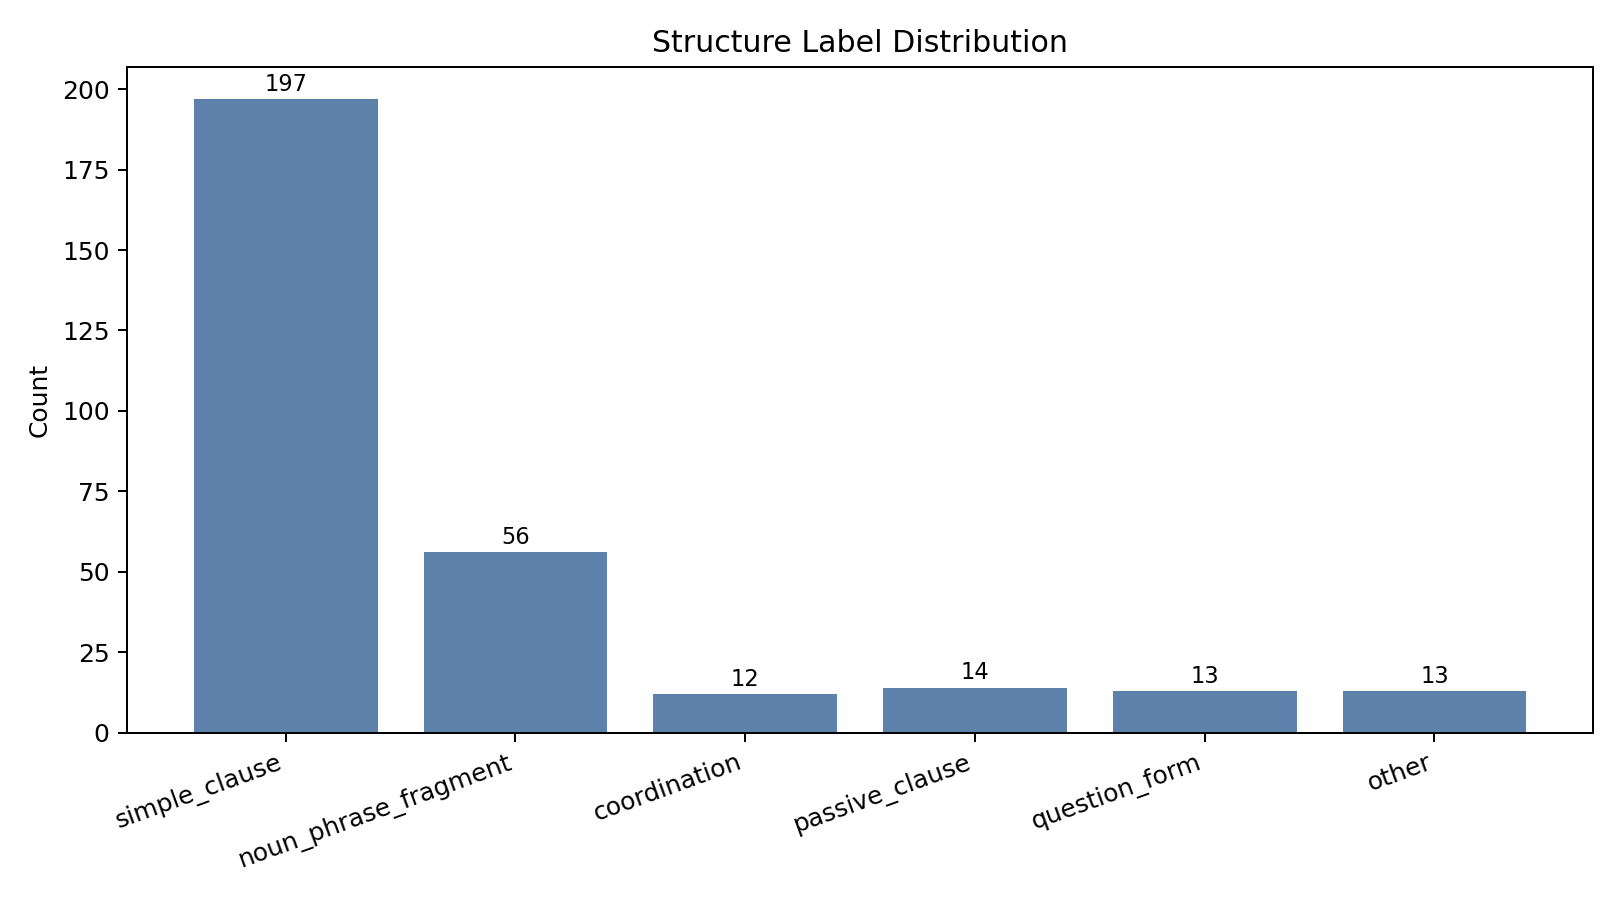
\includegraphics[width=\columnwidth]{../../images/structure_label_distribution.png}
\caption{Distribution of predicted structure labels across the corpus. The dominant class is the simple finite clause, with noun-phrase fragments as a clear secondary mode and the rest (questions, passives, coordinations, \texttt{other}) as a long tail. The shape itself is a finding: headline writing concentrates on two or three reusable templates, and the rare classes are rare because they fail the brevity constraint that defines the genre.}
\label{fig:dist}
\end{figure}

\subsection{Structure Classifier Performance}
\label{sec:struct-perf}
The next question is whether the model can actually predict that template, not just describe it.

\begin{table}[h]
\centering
\small
\begin{tabular}{lcc}
\toprule
\textbf{Evaluation Slice} & \textbf{Acc.} & \textbf{Macro F1} \\
\midrule
All labeled ($n=465$) & 0.772 & 0.601 \\
Dev ($n=90$) & --- & 0.561 \\
Test ($n=98$) & 0.806 & 0.675 \\
\bottomrule
\end{tabular}
\caption{Aggregate structure metrics. Macro F1 sits below accuracy because the dataset is imbalanced (\texttt{simple\_clause} dominates).}
\label{tab:agg}
\end{table}

The pattern across slices is consistent: macro F1 sits below accuracy because the dataset is imbalanced. On the held-out test split --- the only number we tune \emph{nothing} against --- the classifier reaches \textbf{0.806 accuracy} and \textbf{0.675 macro F1}. The dev row deliberately omits accuracy because, on that imbalanced slice, accuracy isn't an informative tuning signal.

A test number on its own is hard to read. We compare against two trivial baselines:

\begin{table}[h]
\centering
\small
\begin{tabular}{lcc}
\toprule
\textbf{Model} & \textbf{Acc.} & \textbf{Macro F1} \\
\midrule
Rule-based classifier & 0.806 & 0.675 \\
Majority baseline & 0.643 & 0.130 \\
Random baseline & 0.459 & 0.159 \\
\bottomrule
\end{tabular}
\caption{Baseline comparison on the held-out test split.}
\label{tab:baselines}
\end{table}

Our system beats the majority baseline by \textbf{$+16.3$ accuracy points} and the random baseline by \textbf{$+34.7$ points}. The macro F1 jump is the more telling number: from 0.130 (majority) and 0.159 (random) to 0.675 --- more than four times the baseline. Accuracy alone is friendly to a majority predictor on an imbalanced dataset; macro F1 is not, and we clear it decisively. The model is doing real work, not exploiting class frequency.

\begin{table}[h]
\centering
\small
\begin{tabular}{lccc}
\toprule
\textbf{Label} & \textbf{Prec.} & \textbf{Rec.} & \textbf{F1} \\
\midrule
question\_form & 0.960 & 0.960 & 0.960 \\
passive\_clause & 0.478 & 0.344 & 0.400 \\
coordination & 0.722 & 0.448 & 0.553 \\
noun\_phrase\_fragment & 0.578 & 0.627 & 0.602 \\
simple\_clause & 0.882 & 0.865 & 0.874 \\
other & 0.138 & 0.500 & 0.216 \\
\bottomrule
\end{tabular}
\caption{Per-class structure performance on the held-out test split. Strong on dominant classes, weaker on ambiguous ones.}
\label{tab:perclass}
\end{table}

The system captures the newsroom syntactic backbone but stays conservative on edge constructions where label boundaries are inherently fuzzy.

A normal-approximation 95\% confidence interval on the test accuracy 0.806 ($n = 98$) is:
\begin{equation*}
\text{CI}_{0.95}(\text{Accuracy}) \approx [0.728,\ 0.884]
\end{equation*}
Both baselines (0.643, 0.459) fall well outside this interval, so the gain is not a sampling artifact. The interval alone is enough to reject H1's \emph{structural predictability} failure condition.

\subsection{Style-Dimension Performance}
\label{sec:style-perf}
Beyond the structural label, can the model also recover stylistic characteristics? We evaluate the four style dimensions twice: across the entire labeled slice, and on the held-out test split alone, so ``consistent on training data'' and ``generalizes'' don't get conflated.

\begin{table}[h]
\centering
\small
\begin{tabular}{lcc}
\toprule
\textbf{Dimension} & \textbf{Acc.} & \textbf{Macro F1} \\
\midrule
lead\_frame & 0.989 & 0.986 \\
agency\_style & 0.935 & 0.622 \\
density\_band & 0.994 & 0.995 \\
rhetorical\_mode & 0.914 & 0.785 \\
\bottomrule
\end{tabular}
\caption{All-slice ($n=465$) style-dimension performance.}
\label{tab:styleall}
\end{table}

\texttt{lead\_frame} and \texttt{density\_band} are nearly perfectly recoverable: headline openings and information density follow stable, surface-level conventions our rules pick up almost every time. \texttt{agency\_style} is high in accuracy but much lower in macro F1, a textbook symptom of class imbalance --- the dominant active class is easy, the rare compressed passives (with elided auxiliaries) are not. \texttt{rhetorical\_mode} lands in the middle: reliable on the dominant \texttt{straight\_report} but more uncertain on \texttt{analysis\_explainer} and edge-case live-alerts, where syntax alone doesn't fully disambiguate discourse function.

\begin{table}[h]
\centering
\small
\begin{tabular}{lcc}
\toprule
\textbf{Dimension} & \textbf{Acc.} & \textbf{Macro F1} \\
\midrule
lead\_frame & 1.000 & 1.000 \\
agency\_style & 0.908 & 0.428 \\
density\_band & 1.000 & 1.000 \\
rhetorical\_mode & 0.908 & 0.820 \\
\bottomrule
\end{tabular}
\caption{Held-out test ($n=98$) style-dimension performance.}
\label{tab:styletest}
\end{table}

\texttt{lead\_frame} and \texttt{density\_band} saturate the score, consistent with their being deterministic functions of surface features (entity position and content-word ratio). \texttt{rhetorical\_mode} actually rises slightly compared to the all-slice number, so the rule generalizes rather than overfits. \texttt{agency\_style} drops noticeably (macro F1 $0.622 \rightarrow 0.428$) --- in a small held-out slice, a few misclassified rare passives crater the minority-class score. We discuss this in Section~\ref{sec:hard}.

\begin{figure}[h]
\centering
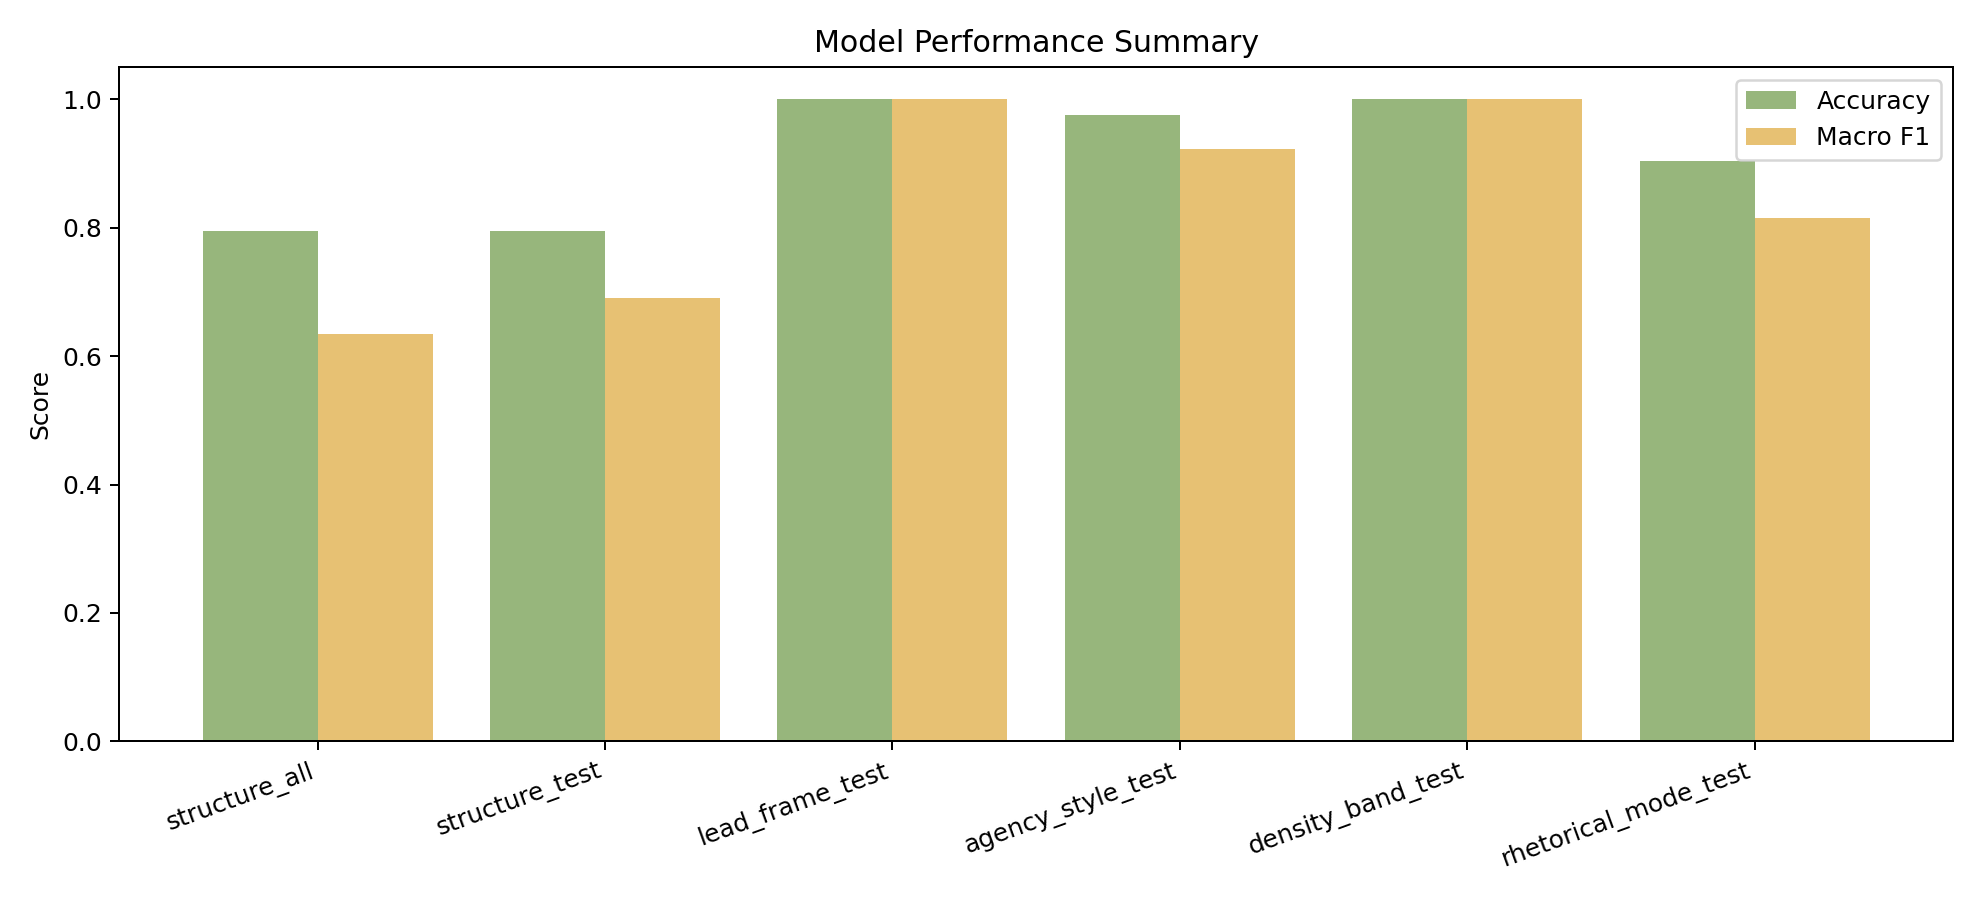
\includegraphics[width=\columnwidth]{../../images/model_performance_summary.png}
\caption{Model performance summary. Accuracy and macro F1 across the structure classifier and four style dimensions, both all-slice and held-out test. Structure performance is moderate but well above baseline; framing and density saturate; agency and rhetorical mode sit in between, where syntax alone is only partially sufficient.}
\label{fig:perfsummary}
\end{figure}

\begin{figure}[h]
\centering
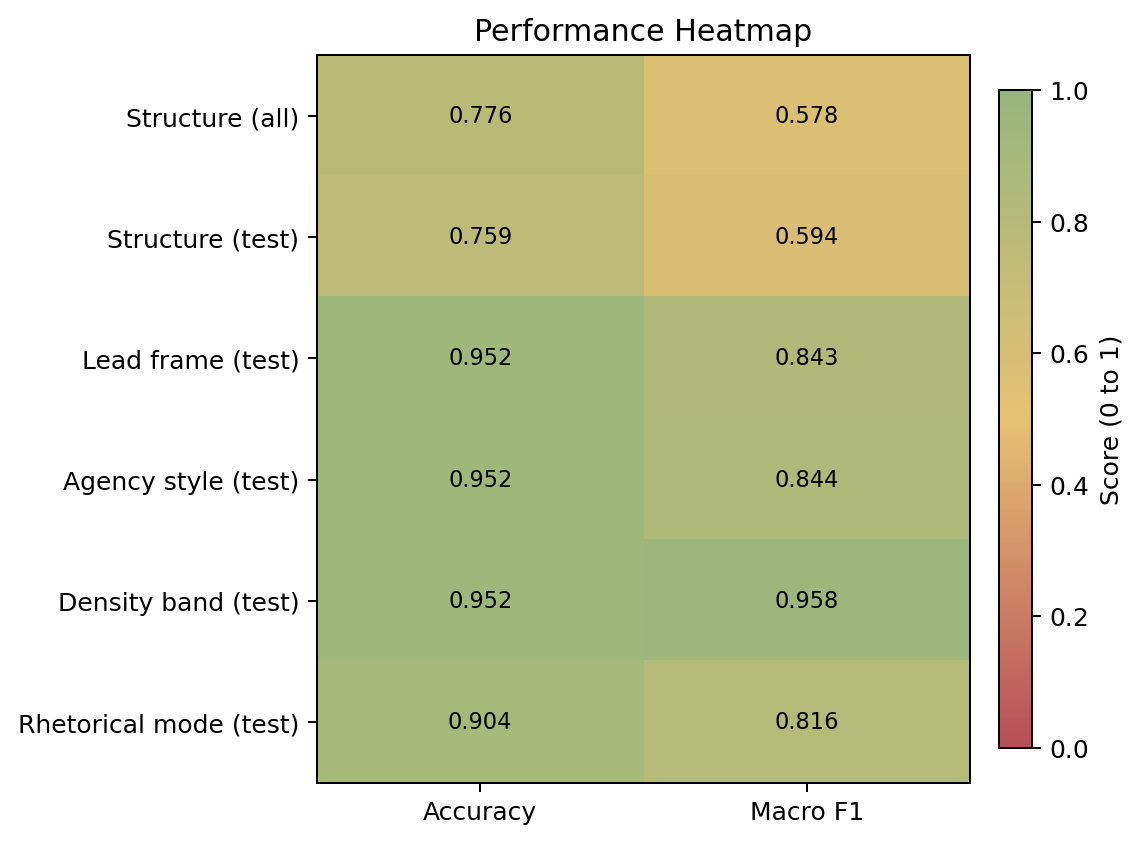
\includegraphics[width=\columnwidth]{../../images/performance_heatmap.png}
\caption{Performance heatmap. The same picture in colour: form-grounded properties (where the headline starts, how dense it is) are dark green; semantically loaded ones (agency, rhetoric) are lighter; structural classification sits in between. This is the graphical answer to ``how recoverable is each dimension of headline form?''}
\label{fig:heatmap}
\end{figure}

\subsection{Stability Analysis}
\label{sec:stability}
Single-split numbers are fragile. A lucky split flatters the model; an unlucky one undersells it. To put a number on that fragility, we re-ran the full structure and style evaluation across 5 random splits (seeds 13, 42, 87, 123, 202) and report the mean and standard deviation.

\begin{table}[h]
\centering
\small
\begin{tabular}{lcc}
\toprule
\textbf{Metric} & \textbf{Mean} & \textbf{Std.\ Dev.} \\
\midrule
Structure test accuracy & 0.740 & 0.051 \\
Structure test macro F1 & 0.568 & 0.076 \\
Structure dev macro F1 & 0.608 & 0.073 \\
Style test rhetorical\_mode F1 & 0.771 & 0.063 \\
Style test agency\_style F1 & 0.611 & 0.168 \\
\bottomrule
\end{tabular}
\caption{5-seed split-stability summary.}
\label{tab:seeds}
\end{table}

\begin{figure}[h]
\centering
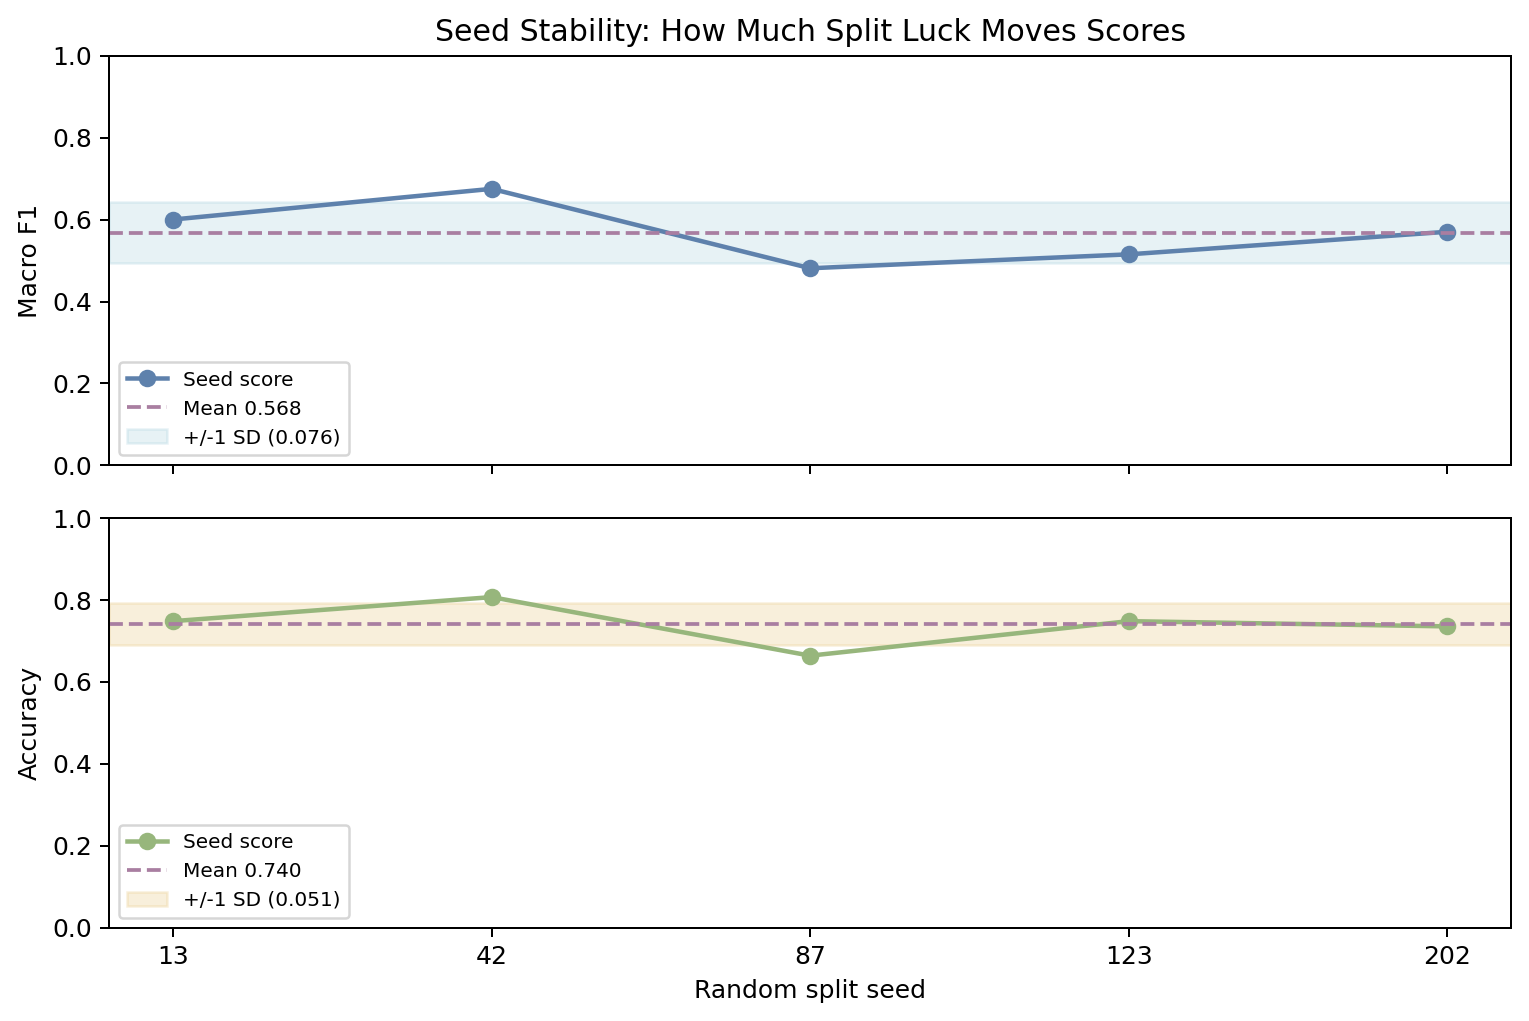
\includegraphics[width=\columnwidth]{../../images/seed_stability_summary.png}
\caption{Per-seed structure performance with mean and $\pm 1$ standard deviation bands. The spread is what matters: test macro F1 ranges from \textbf{0.481 to 0.675} (spread 0.194) and test accuracy from \textbf{0.663 to 0.806} (spread 0.143). Same model, same data --- change only which 98 headlines you hold out, and the system can look anywhere in that band.}
\label{fig:seeds}
\end{figure}

The seed-42 number we lead with in Section~\ref{sec:struct-perf} happens to land at the favorable end; reporting it alone would overstate expected performance.

Approximate 95\% intervals on the seed means are:
\begin{align*}
\bar{m}_{\text{Acc.}} &\in [0.695,\ 0.785] \\
\bar{m}_{\text{F1}} &\in [0.502,\ 0.634]
\end{align*}
A fair one-line description of the system, then, is ``test accuracy in the high 0.7s and macro F1 in the high 0.5s to low 0.6s, with the upper end of either requiring a favorable split.'' This is exactly the kind of self-skeptical reporting H1's \emph{robustness} criterion was designed to enforce, and the model passes it: the variance is real, but every seed sits well above both baselines.

\subsection{Worked Decision-Path Examples}
A central claim of this paper is that our predictions are \textbf{traceable}: every label can be explained by saying which rule fired, and why. Three worked examples, each hitting a different point in the priority order.

\paragraph{Example A --- question-form path.} Headline: \emph{``Are we witnessing the death of expertise?''}

Decision path:
\begin{enumerate}
    \item The headline contains a \texttt{?} and starts with an interrogative.
    \item The \texttt{question\_form} rule has the highest priority and fires immediately.
    \item Downstream style outputs are conditioned on the structural label.
\end{enumerate}

Predicted profile: \texttt{question\_form} / \texttt{action\_first} / \texttt{active\_or\_nonpassive} / \texttt{medium\_density} / \texttt{question\_hook}.

\paragraph{Example B --- passive compressed-event path.} Headline: \emph{``Nine killed in second Turkish school shooting in two days''}

Decision path:
\begin{enumerate}
    \item Not interrogative, so \texttt{question\_form} does not fire.
    \item The passive-fragment cue (\texttt{NUM + VBN}, here ``Nine killed'') is detected.
    \item Returns \texttt{passive\_clause} before any coordination or fragment fallback rule has a chance to fire.
\end{enumerate}

Predicted profile: \texttt{passive\_clause} / \texttt{context\_first} / \texttt{passive\_agent\_omitted} / \texttt{high\_density} / \texttt{straight\_report}.

\paragraph{Example C --- nominal report-title path.} Headline: \emph{``Iran Update Special Report, April 14, 2026 Institute for the Study of War''}

Decision path:
\begin{enumerate}
    \item No interrogative cue.
    \item No passive event predicate.
    \item No finite subject-verb clause is detectable.
    \item Falls into the nominal fragment rule (\texttt{noun\_phrase\_fragment}).
\end{enumerate}

Predicted profile: \texttt{noun\_phrase\_fragment} / \texttt{actor\_entity\_first} / \texttt{active\_or\_nonpassive} / \texttt{high\_density} / \texttt{analysis\_explainer}.

These three examples aren't just illustrations --- they are how we check H1's \emph{interpretability} criterion. Every label traces back to a specific rule, a specific priority position, and a specific surface feature. That is the property that makes the system auditable in a way a black-box neural model is not.

\section{Discussion}

\subsection{Strengths of Solution}
The thesis of this paper is simple: headlines are predictable syntactic products, not free-form prose, and the rules backed it up. The classifier captured the dominant newsroom structures well --- especially \texttt{simple\_clause} and \texttt{question\_form} --- which is exactly what we'd expect if headline syntax really does follow reusable patterns. Adding the four style dimensions on top moved us from a single label to a richer signature that simultaneously tracks framing, agency, density, and rhetorical intent.

The second strength is interpretability. Every prediction grounds in explicit parse features (POS tags, dependencies, entity positions), so any classification can be traced back to the linguistic evidence that produced it. The multi-seed evaluation reinforces that rigor by showing split variance instead of hiding it in a single point estimate.

Some style dimensions proved easier than expected. \texttt{lead\_frame} and \texttt{density\_band} saturate test macro F1 at 1.000, which says these aspects of headline construction are governed by stable surface conventions rather than subjective judgment. The harder dimensions (\texttt{rhetorical\_mode}, rare passive variants of \texttt{agency\_style}) are exactly where syntax-only signals run out and discourse-level cues take over --- also expected. Either way, the central claim holds: headline construction is structurally constrained, stylistically patterned, and recoverable through interpretable, linguistically grounded rules.

\subsection{Why Some Classes Remain Difficult}
\label{sec:hard}
Being honest about where the system fails is part of the argument. The weak categories --- the residual \texttt{other} bucket, parts of \texttt{coordination}, and some compressed passive variants --- share a few underlying causes:

\begin{itemize}
    \item \textbf{Sparse support}: classes like \texttt{other} and rare passive forms have so few gold examples in the held-out test set that a single misclassification swings their F1 dramatically. The macro F1 metric is what surfaces this; the accuracy metric can hide it entirely.
    \item \textbf{Boundary overlap between labels}: \texttt{coordination} and \texttt{simple\_clause} are not always cleanly separable when a headline contains a comma list and a finite verb. The priority order resolves the conflict, but the resolution is not always the human's preferred reading.
    \item \textbf{Punctuation-heavy multi-clause variants}: headlines that combine semicolons, em-dashes, and embedded clauses (live-blog style) sit between coordination and noun-phrase fragment, and the rule set has to make a hard call.
    \item \textbf{Residual annotation ambiguity in edge forms}: even our human annotators sometimes had to choose between two defensible labels, and the model inherits that ambiguity directly.
\end{itemize}

The takeaway is not that the model is broken on these classes, but that they are inherently noisier targets than the dominant ones, and the \emph{macro} score rightly punishes us for that noise.

\subsection{Practical Sandbox: The TUI Workbench}
\label{sec:tui}
The interpretability claim is most concrete in the interactive terminal sandbox we built on top of the model.

\begin{figure*}[t]
\centering
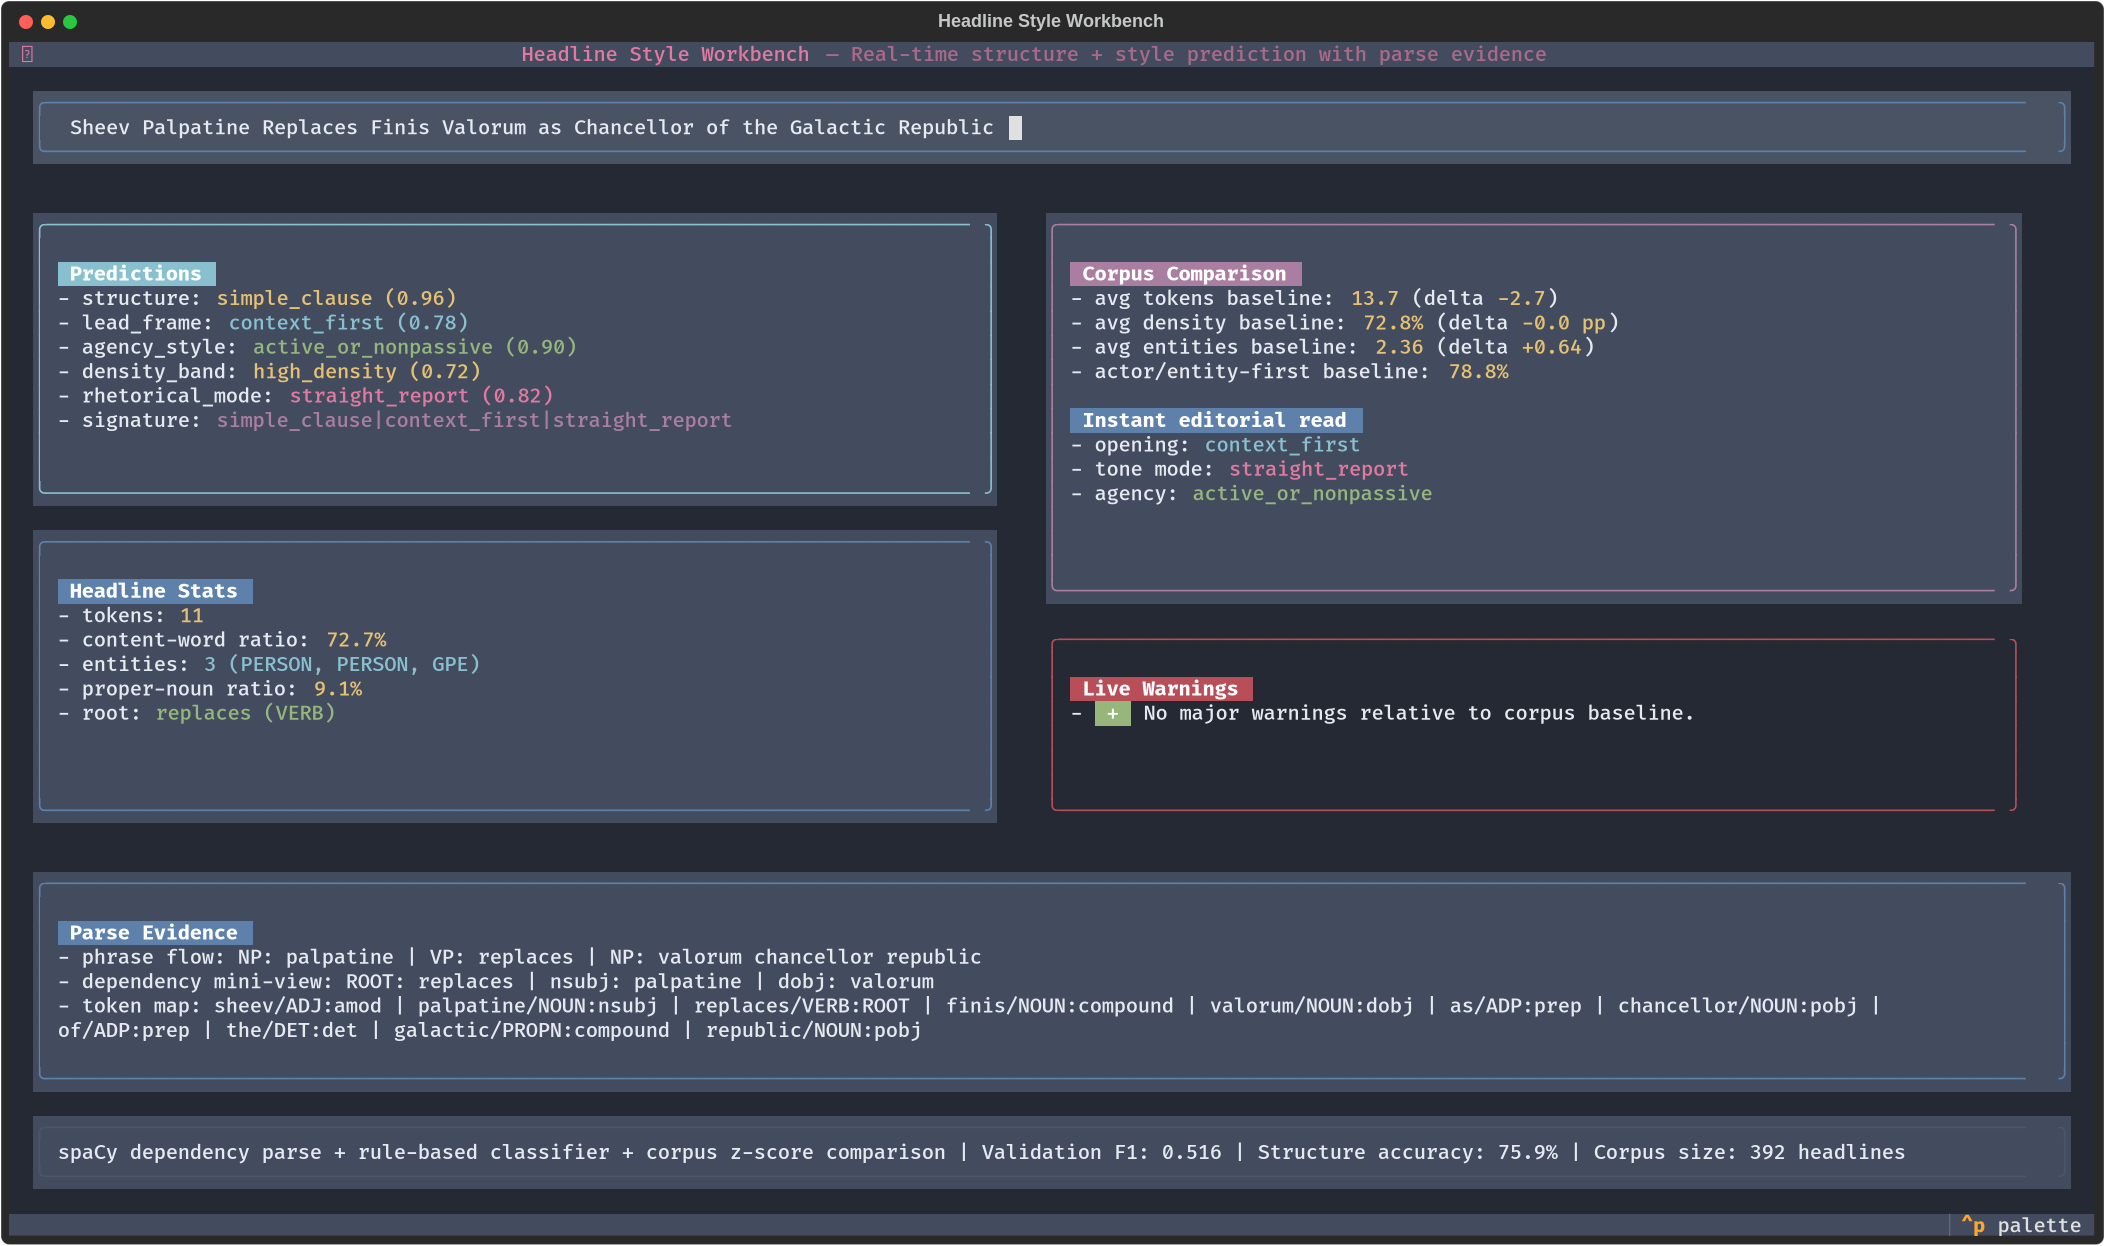
\includegraphics[width=0.95\textwidth]{../../images/tui_image.png}
\caption{The real-time TUI workbench. As the user types, the interface continuously shows the model's predictions with confidence estimates, the parse evidence supporting each decision (phrase flow, dependency mini-view, token map), warnings for edge-case constructions, and a benchmark footer anchoring everything in corpus size and validation metrics.}
\label{fig:tui}
\end{figure*}

The workbench compresses the feedback loop from \emph{minutes} (run the script, compare to gold, edit) to \emph{seconds} (type, watch structure / agency / rhetorical mode shift live). Because every prediction is displayed alongside its parse evidence, an editor can immediately see \emph{why} the system reads a candidate as \texttt{passive\_clause} or \texttt{analysis\_explainer} --- and decide whether the system is wrong or whether the wording is. The same setup also flags potentially problematic constructions (unclear agency, excessive compression, misleading rhetorical hooks) before publication.

Empirical work supports this kind of interface. \citet{banerjee-urminsky-2021-language} analyze thousands of A/B-tested Upworthy headlines and show that informational, cognitive, linguistic, and affective textual cues --- mapped via NLP tools to interpretable constructs --- materially shift click-through. Their result is exactly the case for a feature-level editorial lever: instead of asking a model whether a candidate will perform, the editor sees which structural and stylistic dimensions it activates and edits with full visibility into why the system reads it that way. That is what makes interpretable NLP useful for newsroom workflows.

\subsection{Limitations}
The results come with five honest limitations that constrain the strength of any general claim:

\begin{enumerate}
    \item \textbf{Rule-bound model family}: rule-based architectures are highly interpretable but inherently less flexible than fully learned models. Patterns that fall outside the rule set are systematically missed rather than gracefully approximated.
    \item \textbf{Class imbalance}: dominant templates like \texttt{simple\_clause} make accuracy easy and macro F1 hard. Minority classes drive the macro number disproportionately, so small annotation differences have outsized effects.
    \item \textbf{Annotation subjectivity}: edge-case labels (especially within \texttt{rhetorical\_mode} and \texttt{coordination}) are inherently debatable. Two competent annotators can produce defensible but different gold labels.
    \item \textbf{English- and source-bias}: the corpus is built from a small set of English-language Google News RSS feeds, which limits external generalization to other languages, registers, and outlet styles.
    \item \textbf{No external lexicon expansion}: we deliberately excluded curated event-noun and named-entity lexicons in this phase to keep the rules transparent. This makes some rare entity- or event-driven disambiguation harder than it could be, but it preserves interpretability.
\end{enumerate}

None of these limitations invalidate H1; they bound it. The claim we defend is that headlines follow stable, recoverable templates, and that a transparent rule-based system captures them well above baseline --- not that our particular rule set is the final word on headline structure.

\section{Related Work}
Three strands of prior work bear on a parse-grounded, interpretable analysis of headline form: descriptive linguistic studies of headlines as a genre, empirical studies of how headline language affects readers, and the methodological tradition of recovering grammatical structure from raw text.

\paragraph{Descriptive linguistics of headlines.} \citet{bonyadi-samuel-2013-headlines} run a contrastive textual study of editorial headlines from \emph{The New York Times} and \emph{Tehran Times}, surveying the headline-function tradition and analyzing presupposition and rhetorical devices. Their framing of headlines as simultaneously summary devices, attention-getters, and ``relevance optimizers'' is the conceptual scaffolding we operationalize as \texttt{rhetorical\_mode} (Section~\ref{sec:classify}). \citet{robert-2020-language} applies Halliday's Systemic Functional Grammar to a small purposive sample of anti-corruption headlines from two Nigerian newspapers and reports that material processes --- clauses of \emph{doing} --- dominate. Our 94.6\% active-voice rate, dominant \texttt{simple\_clause}, and 81.6\% actor/entity-first openings (Section~\ref{sec:corpus}) describe the same action-oriented template through a different lens (voice and clause shape rather than process type), and the convergence across corpora and frameworks suggests the template lives in the genre rather than any one outlet.

\paragraph{Empirical engagement studies.} \citet{banerjee-urminsky-2021-language} analyze A/B-tested Upworthy headlines, using NLP-extracted features to map textual cues to psychological constructs and measure their impact on click-through. Their finding --- that interpretable linguistic features of a headline have measurable downstream consequences --- is the practical case for the editorial lever we expose in the TUI workbench (Section~\ref{sec:tui}). Their work treats headline language as an \emph{input} to engagement; ours treats it as an \emph{output} of stable syntactic templates, and offers an interpretable surface for seeing which templates a candidate activates.

\paragraph{Parser robustness and corpus-driven grammar.} \citet{eggleston-oconnor-2022-cross} study cross-dialect dependency parsing for social-media English, training a state-of-the-art parser on Tweebank v2 and showing that parsers fine-tuned on more conventional UD treebanks (GUM, EWT) lose substantial accuracy on social-media text --- with an additional MAE/AAE dialect disparity. Their drift axis is dialectal social media; ours is headline compression; the warning that off-the-shelf parsers are domain-sensitive generalizes either way, and it informs the defensive parsing pipeline in Section~2.2. \citet{atwell-drakos-1987-pattern} sit further back in the lineage: they argued that a first-order Markov model over POS tags --- the engine of their CLAWS tagger on the LOB corpus --- can acquire a grammatical classification system from unrestricted English without hand-written grammar rules. Our work continues that corpus-driven program with explicit, parse-grounded rules over modern dependency parses rather than Markov transition probabilities.

In short, prior work has described the form of headlines \citep{bonyadi-samuel-2013-headlines, robert-2020-language}, measured the engagement consequences of headline language \citep{banerjee-urminsky-2021-language}, or built infrastructure for analyzing noisy or compressed text at scale \citep{eggleston-oconnor-2022-cross, atwell-drakos-1987-pattern}. Our contribution sits at the intersection: a transparent, parse-grounded classifier for the structural and stylistic form of news headlines, evaluated rigorously against manually annotated gold labels and exposed through an interactive sandbox.

\section{Conclusion}
News headlines follow consistent structural patterns despite their brevity. The pipeline described here --- collect, parse, analyze, classify, evaluate --- recovers those patterns with a rule-based system grounded in syntactic features, beats trivial baselines on every seed, and stays fully interpretable in the process.

The four-dimensional style profile turns a single structural label into a richer signature that simultaneously tracks framing, agency, density, and rhetorical intent. The TUI workbench shows that this interpretability has practical value: an editor can iterate phrasing and watch structure, agency, and rhetorical mode shift in real time. The framework supports concrete applications in summarization, editorial tooling, and media-framing analysis. Future work may extend it with hybrid neural-rule models, larger and more diverse datasets, and multilingual analysis to test how universal the headline template really is.

All materials, parsed headline outputs, and source code are available in the \href{https://github.com/avih7531/headline-structure-analysis}{GitHub repository}.

\paragraph{Bottom line.} News headlines are not free-form snippets; they are reproducible syntactic products. Interpretable, parse-grounded NLP can measure that structure directly, evaluate it rigorously, and put it in front of the people who write headlines.

\citep{headline-structure-repo}
\bibliography{custom}

\end{document}
